\input docmac

\title{Guide to Packaging with Descot}
\author{Shu Zhou and Aaron W. Hsu}
\contact{[shuzhou,awhsu]@indiana.edu}

\maketitlepage

\abstract
This would be an abstract. You should fill it in with all sorts of
goodies and the like. I wonder if when the quick brown fox jumps over
the lazy dog that the white whale will eat Captain Nemo. This would be an abstract. You should fill it in with all sorts of
goodies and the like. I wonder if when the quick brown fox jumps over
the lazy dog that the white whale will eat Captain Nemo. This would be an abstract. You should fill it in with all sorts of
goodies and the like. I wonder if when the quick brown fox jumps over
the lazy dog that the white whale will eat Captain Nemo. This would be an abstract. You should fill it in with all sorts of
goodies and the like. I wonder if when the quick brown fox jumps over
the lazy dog that the white whale will eat Captain Nemo. 
\endabstract

\chapter{This is a chapter}{chp-whatever}%
This is what a chapter will look like without any thing like this. This
might be interesting. This is what a chapter will look like without any thing like this. This
might be interesting. This is what a chapter will look like without any thing like this. This
might be interesting. This is what a chapter will look like without any thing like this. This
might be interesting. This is what a chapter will look like without any thing like this. This
might be interesting. This is what a chapter will look like without any thing like this. This
might be interesting. This is what a chapter will look like without any thing like this. This
might be interesting. This is what a chapter will look like without any thing like this. This
might be interesting. This is what a chapter will look like without any thing like this. This
might be interesting. This is what a chapter will look like without any thing like this. This
might be interesting.

\chapter{Next Chapter}{other-index}%

\section{This is a section heading}{sec-samp}%
This is what we would do if we want to put a section in here. We could
also put something like the next in as well. This is what we would do if we want to put a section in here. We could
also put something like the next in as well. This is what we would do if we want to put a section in here. We could
also put something like the next in as well. This is what we would do if we want to put a section in here. We could
also put something like the next in as well. This is what we would do if we want to put a section in here. We could
also put something like the next in as well. This is what we would do if we want to put a section in here. We could
also put something like the next in as well. 

This is what we would do if we want to put a section in here. We could
also put something like the next in as well. This is what we would do if we want to put a section in here. We could
also put something like the next in as well. This is what we would do if we want to put a section in here. We could
also put something like the next in as well. This is what we would do if we want to put a section in here. We could
also put something like the next in as well. This is what we would do if we want to put a section in here. We could
also put something like the next in as well. This is what we would do if we want to put a section in here. We could
also put something like the next in as well. 

\medskip{\narrower\noindent
This is a quote from someone famous. This is a quote from someone
famous. This is a quote from someone famous. This is a quote from
someone famous. This is a quote from someone famous. This is a quote
from someone famous. This is a quote from someone famous. This is a
quote from someone famous.\par}\medskip

\noindent This is the next paragraph.

\medskip\verbatim
$ tex sample_doc.tex
  And it obeys indenting and ignores \funny things.
|endverbatim

\section{Subbed Section}{sec-sub-samp}%
\subsection{Real Subsection}{sub-sec-samp}%
This would contain the contents of the sub section.

You could also put a graphic somewhere in ehre.

\figplace{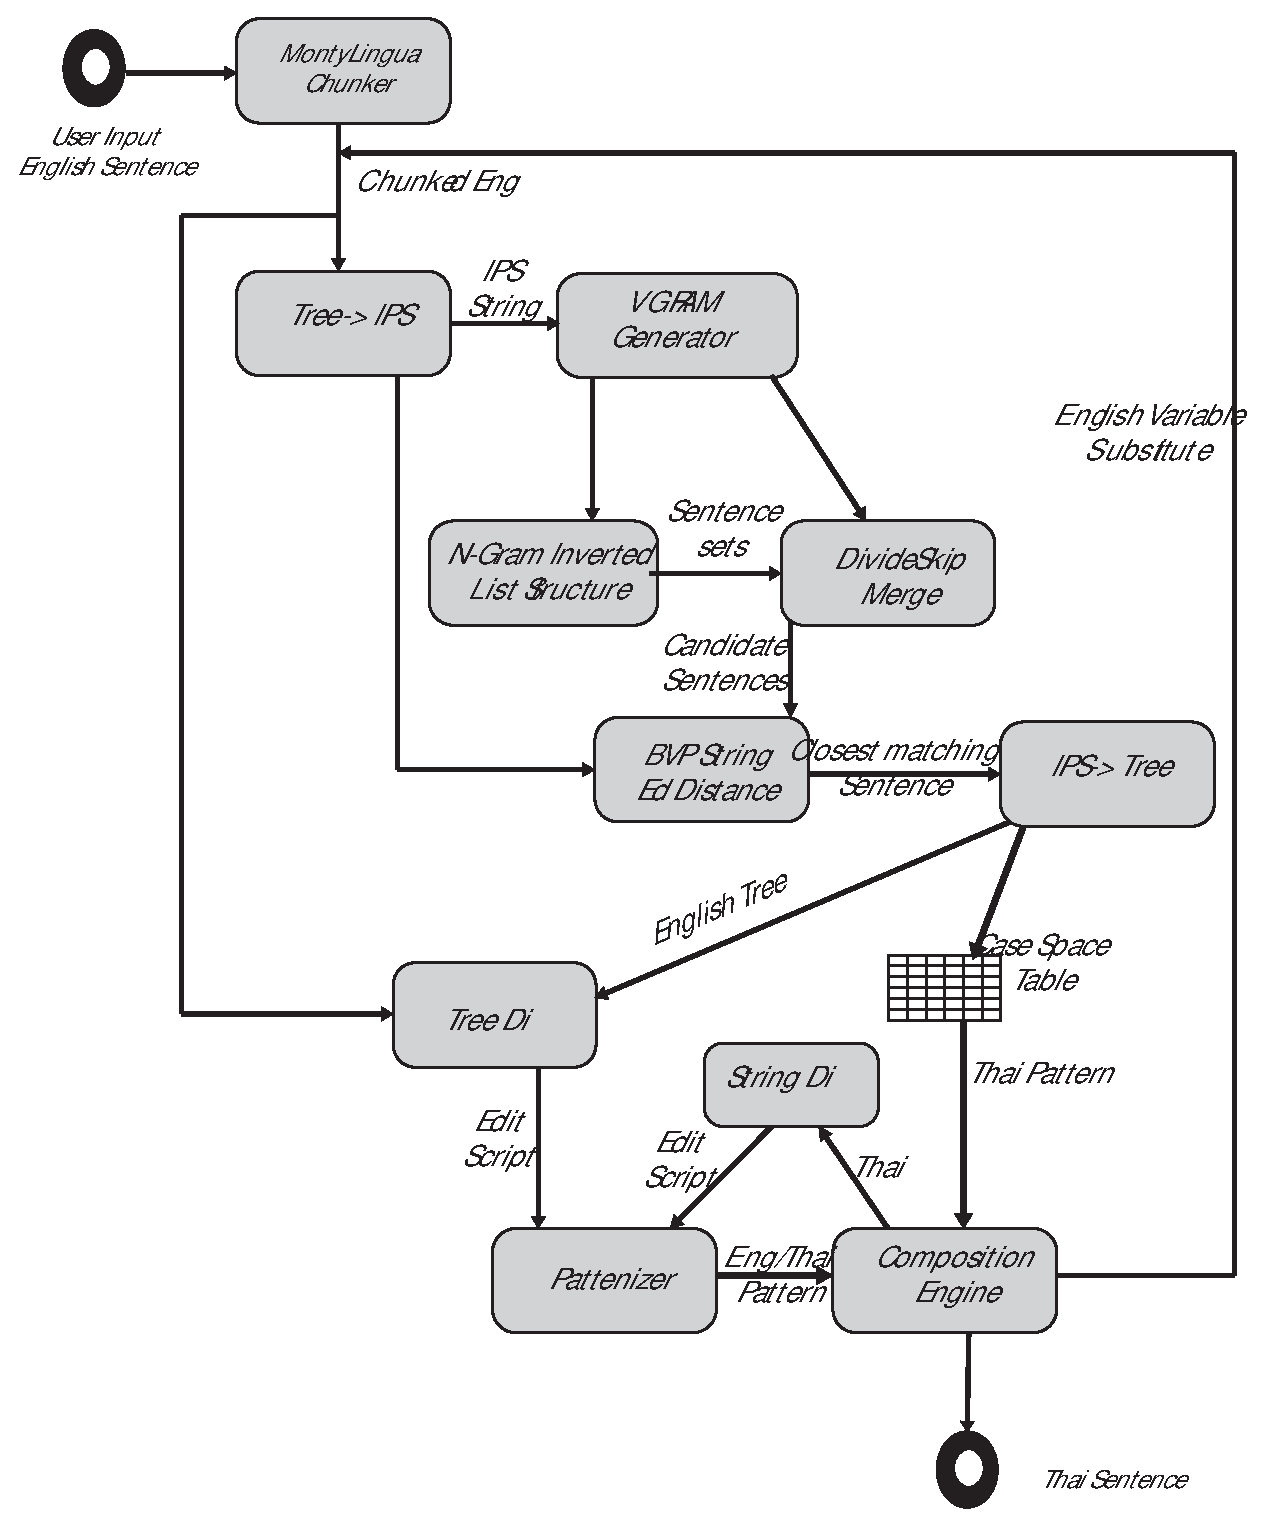
\includegraphics[width=15cm]{overview.eps}}
  {Workflow Outline}
  {Workflow Outline}

\bye
